\documentclass[a4paper, twocolumn]{article}
\setlength{\columnsep}{40pt}
\usepackage{graphicx} 
\usepackage[a4paper,margin=0.5in]{geometry}
\usepackage{amsmath}
\usepackage{booktabs}
\usepackage{float}

\title{Dimensionality Reduction and Hypothesis Testing}
\author{Jawadul Chowdhury}
\date{\today}


\begin{document}

\setlength{\intextsep}{0pt} 
\setlength{\textfloatsep}{5pt} 

\maketitle
\onecolumn

\tableofcontents
\newpage

\twocolumn


\section{Introduction}
In this section, we discuss about what the paper is about as well as the kind of dataset we use, as well as the features and how big the dataset is.

\subsection{Abstract}
In this paper, we analyze 63,542 emails. We convert the raw text from these emails into a feature matrix using a  "bag of words" model. Each column of the 
feature matrix corresponds to one word, each row corresponds to one email,  and the entry stores the number of times that word was found in the email. We 
then perform dimensionality reduction, cluster the emails in two clusters. Lastly, we perform binomial testing on all words in each cluster and filter
out the top 200 words.

\subsection{About the Dataset}
Using the 63,452 emails, we converted them into a pandas data frame. A closer look at the pandas data frame tells us that it consists of 5 
features, which are \texttt{category}, \texttt{to\_address}, \texttt{from\_address}, \texttt{subject} and \texttt{body}. The dataset consists of 63542 rows
and 5 columns. For the experiments we perform on the dataset, we are primarily concerned with the \texttt{category} and \texttt{body}, as will be seen in the
sections below.

\section{Method}
In this section, we discuss the methods we used to perform dimensionality reduction and feature extraction. We discuss in detail all the steps that were 
performed and why they were performed. The purpose of this section is detail the steps and explain the concepts behind what we did.

\subsection{Feature Extraction}
Throughout the course of this lab, we extract all the emails that we have stored in a directory from a .json format into a pandas data frame. We then 
perform feature extraction, where we create a feature matrix from the text that makes up the body of the email. We ensure that we only capture words that are
mentioned more than 10 times. The reason we do this is because we would like to reduce noise from rare words as well as prevent overfitting in the 
unsupervised learning model that will be used later on. \\

\noindent Another point worth noting is that when we reduce the number of words, it helps to lower the dimensionality of the data. Lastly, if we were to
include a great number of rare words, this will cause inconsistencies and will disrupt the clustering process when using a unsupervised machine learning
model.

\subsection{Dimensionality Reduction}
With the current feature matrix that we've created, we perform principal component analysis by reducing the number of dimensions in the data. By reducing it
to 10 columns, we have data that is easier to analyze. Next, we obtain the explained variance ratios, which tell us how much variance is retained by each
component after performing dimensionality reduction. 

\subsection{The Clustering Process}
After performing dimensionality reduction, we use unsupervised learning models to perform clustering. The two methods of clustering we use are centroid based
clustering and aggloromerative hierarchial clustering. 

\subsubsection{Centroid Based Clustering}
When it comes to centroid based clustering, we used k-means. K-means works by partitioning a set of data points into K clusters based on their features so 
that data points within the same cluster are more similar to each other than to those in other clusters. Using k-means means we need to determine the value 
of k (number of clusters), and to find the correct value for k, we determine this using the silhouette score.

\subsubsection{Agglorometative Hierarchial Clustering}
Agglorometative Hierarchial Clustering works by building a hierarchy of clusters. It works by starting each data point as its own individual cluster and then
merging the closest cluster at each step, progressively forming larger clusters until all data points belong to one cluster. For the linkage methods, we used
single linkage, which finds the distance between two clusters in the shortest distance between any two points from different clusters.

\subsection{Document Frequencies of Words}
After clustering all the emails, we now analyze the clusters we've created and how the words we've captured play a role in clustering. We achieve this by 
creating a separate matrix for each cluster containing the rows for the points in that cluster. We convert these matrices into a CSC format due to the benefit
that it is optimized for column slicing. Next, we calculate the document frequency of each word in each cluster. We perform document clustering as it allows
us to determine the importance of a word within a cluster and analyze what the cluster represents.

\subsection{Enriched Words with Statistical Testing}
The aim here is to find words that are enriched in each cluster. As a result, we can interpret the themes in the cluster using statistical tests. 

\subsubsection{Using Binomial Testing}
We use binomial testing to know whether a word appears in more emails than expected in one cluster compared to another. The null and alternative hypothesis 
for binomial testing are states as follows:

\begin{itemize}
    \item \textbf{Null Hypothesis:} the relative document frequencies of the observed cluster are less or equal to those of the tested
    \item \textbf{Alternative Hypothesis:} the document frequency is higher in cluster 0 than in cluster 1
\end{itemize}

\noindent At the end of the day, we use statistical testing to avoid bias.

\subsubsection{The Top 200 Words}
We perform binomial testing on all words in each cluster, and then filter out the top 200 words based on their p-value, as the p-value tells us how strong 
the evidence is, and whether to null hypothesis is true or if there isn't enough evidence to back the null hypothesis.

\section{Results}
In this section, we look at the visualizations that have been produced, and discuss these visualization in detail that will better explain the decisions made
behind choosing the k-value, which unsupervised learning model to use and many more.

\subsection{The Explained Variance Ratio}
In a nutshell, the explained variance ratio tells us how much information each principal component captures from the original data. It shows how important
each component is in representing the original data. We plot the explained variance ratios of the components which are derived from reducing the
dimensionality of the feature matrix as shown in Figure 1.

\begin{figure}[H]
    \centering
    \includegraphics[width=\columnwidth]{C:/GitHub/DataScienceMachineLearning/wk_09/plots/ExplainedVarianceRatio.png}
    \caption{Bar Chart of Explained Variance Ratio}
\end{figure}

\vspace{1em}

\noindent When we look at figure 1, it can be seen that the two highest explained variance ratios can be found in component 0 and component 1. 

\subsection{Scatter Plot of Two Components}
Moving on, using the two components with the highest explained variance ratios, we now create a scatter plot where the x-axis is component 1 and the y-axis
and component 2 as shown in figure 2 below.

\begin{figure}[H]
    \centering
    \includegraphics[width=\columnwidth]{C:/GitHub/DataScienceMachineLearning/wk_09/plots/ScatterPlot.png}
    \caption{Scatter Plot of Two Components}
\end{figure}

\vspace{1em}

\noindent When we look at the scatter plot above, it can be clearly seen that there are two clusters, or maybe two groupings. Lets forget the clusters for a
minute. Lets pay attention to the axes. When we plot component 1 against component 2, what we really are doing is that we're visualizing the data in a two 
dimensional area using two components that were extracted via dimensionality reduction. The components are explained as follows:

\begin{itemize}
    \item \textbf{Component 1:} it is the direction in the feature space that accounts for the most variance 
    \item \textbf{Component 2:} it is orthogonal to component 1 and captures the second most variance
\end{itemize}

\subsection{Colored Scatter Plots of Two Components}
\noindent After creating the first scatter plot, we now create a second scatter plot. Using the \texttt{category} feature which consists of just two unique 
values, which are ham and spam, we now color the plots on the scatter plot according to whether they are ham and spam as shown in Figure 3.

\begin{figure}[H]
    \centering
    \includegraphics[width=\columnwidth]{C:/GitHub/DataScienceMachineLearning/wk_09/plots/ScatterPlotColored.png}
    \caption{Scatter Plot of (Ham \& Spam)}
\end{figure}

\vspace{1em}

\noindent When we look at our new scatter plot above, we can see that the ham and spam clusters are intermigled together, which is not quite helpful as we 
would like to have two separate clusters. The intermingling of these two components can be a indication that it is these two components that aren't enough 
to distinguish the categories of ham and spam. 

\subsection{The Silhoutte Score}
Before we have an attempt at making a k-means model, we need to determine the value of k in order to determine the number of clusters we'd like to create.
The silhouette score is a metric used to evaluate the quality of a clustering result.

\noindent It allows us to understand how well each data point fits within 
its assigned cluster compared to other clusters. We create a line graph of the silhouette scores against the values of k as shown in Figure 4 below.

\begin{figure}[H]
    \centering
    \includegraphics[width=\columnwidth]{C:/GitHub/DataScienceMachineLearning/wk_09/plots/SilhouetteLinePlot.png}
    \caption{Line Graph of Silhouette Scores}
\end{figure}

\vspace{1em}

\noindent When we look at the line graph, it can be evidently seen that the best k-value would be 2, as it has the highest silhouette score. As a result, 
we use this k-value when it comes to centroid based and aggloromerative hierarchial clustering.

\subsection{Centroid Based Clustering}
The first unsupervised learning model we use is k-means. Using a k-value of 2, we cluster using the two SVD components. The clustering algorithm labels the 
points so that all points in the same cluster have the same cluster ID. We color the points according to their cluster labels as shown in Figure 5 below.

\begin{figure}[H]
    \centering
    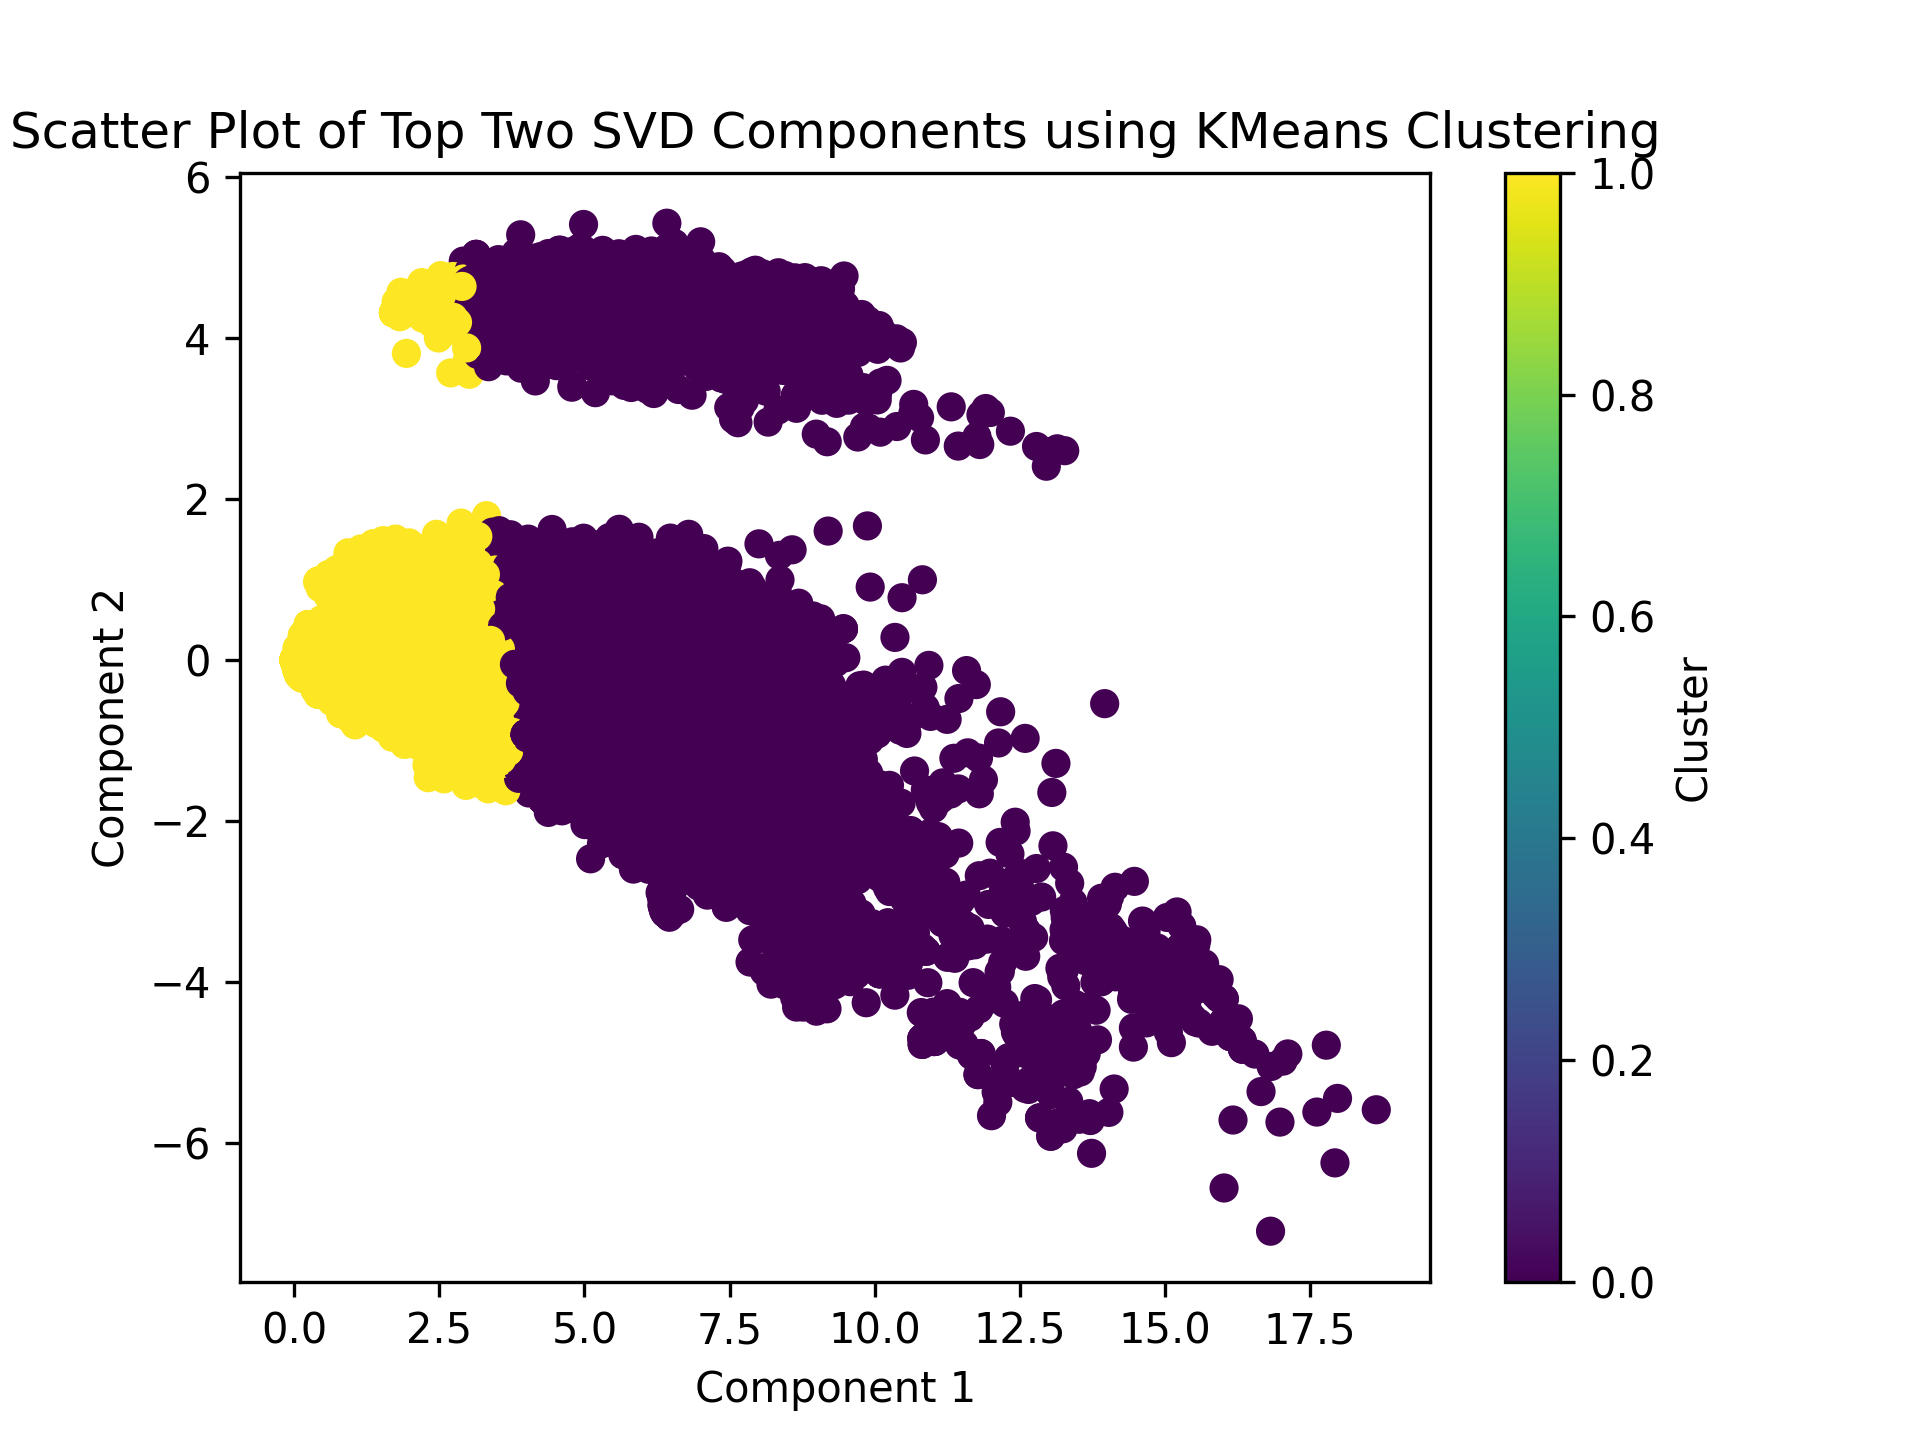
\includegraphics[width=\columnwidth]{C:/GitHub/DataScienceMachineLearning/wk_09/plots/KMeansClustering.png}
    \caption{K-Means Clustering}
\end{figure}

When we look at figure 5, we can tell that the clustering has been done wrong because there is significant overlap between the two clusters, especially 
around the center of the plot. As a result, we turn to aggloromerative hierarchial clustering.

\subsection{Agglorometative Hierarchial Clustering}
The next unsupervised learning model we use is aggloromerative hierarchial clustering. Setting the number of clusters as 2 and the type of linkage as single,
we extract the top two components and produce Figure 6.

\begin{figure}[H]
    \centering
    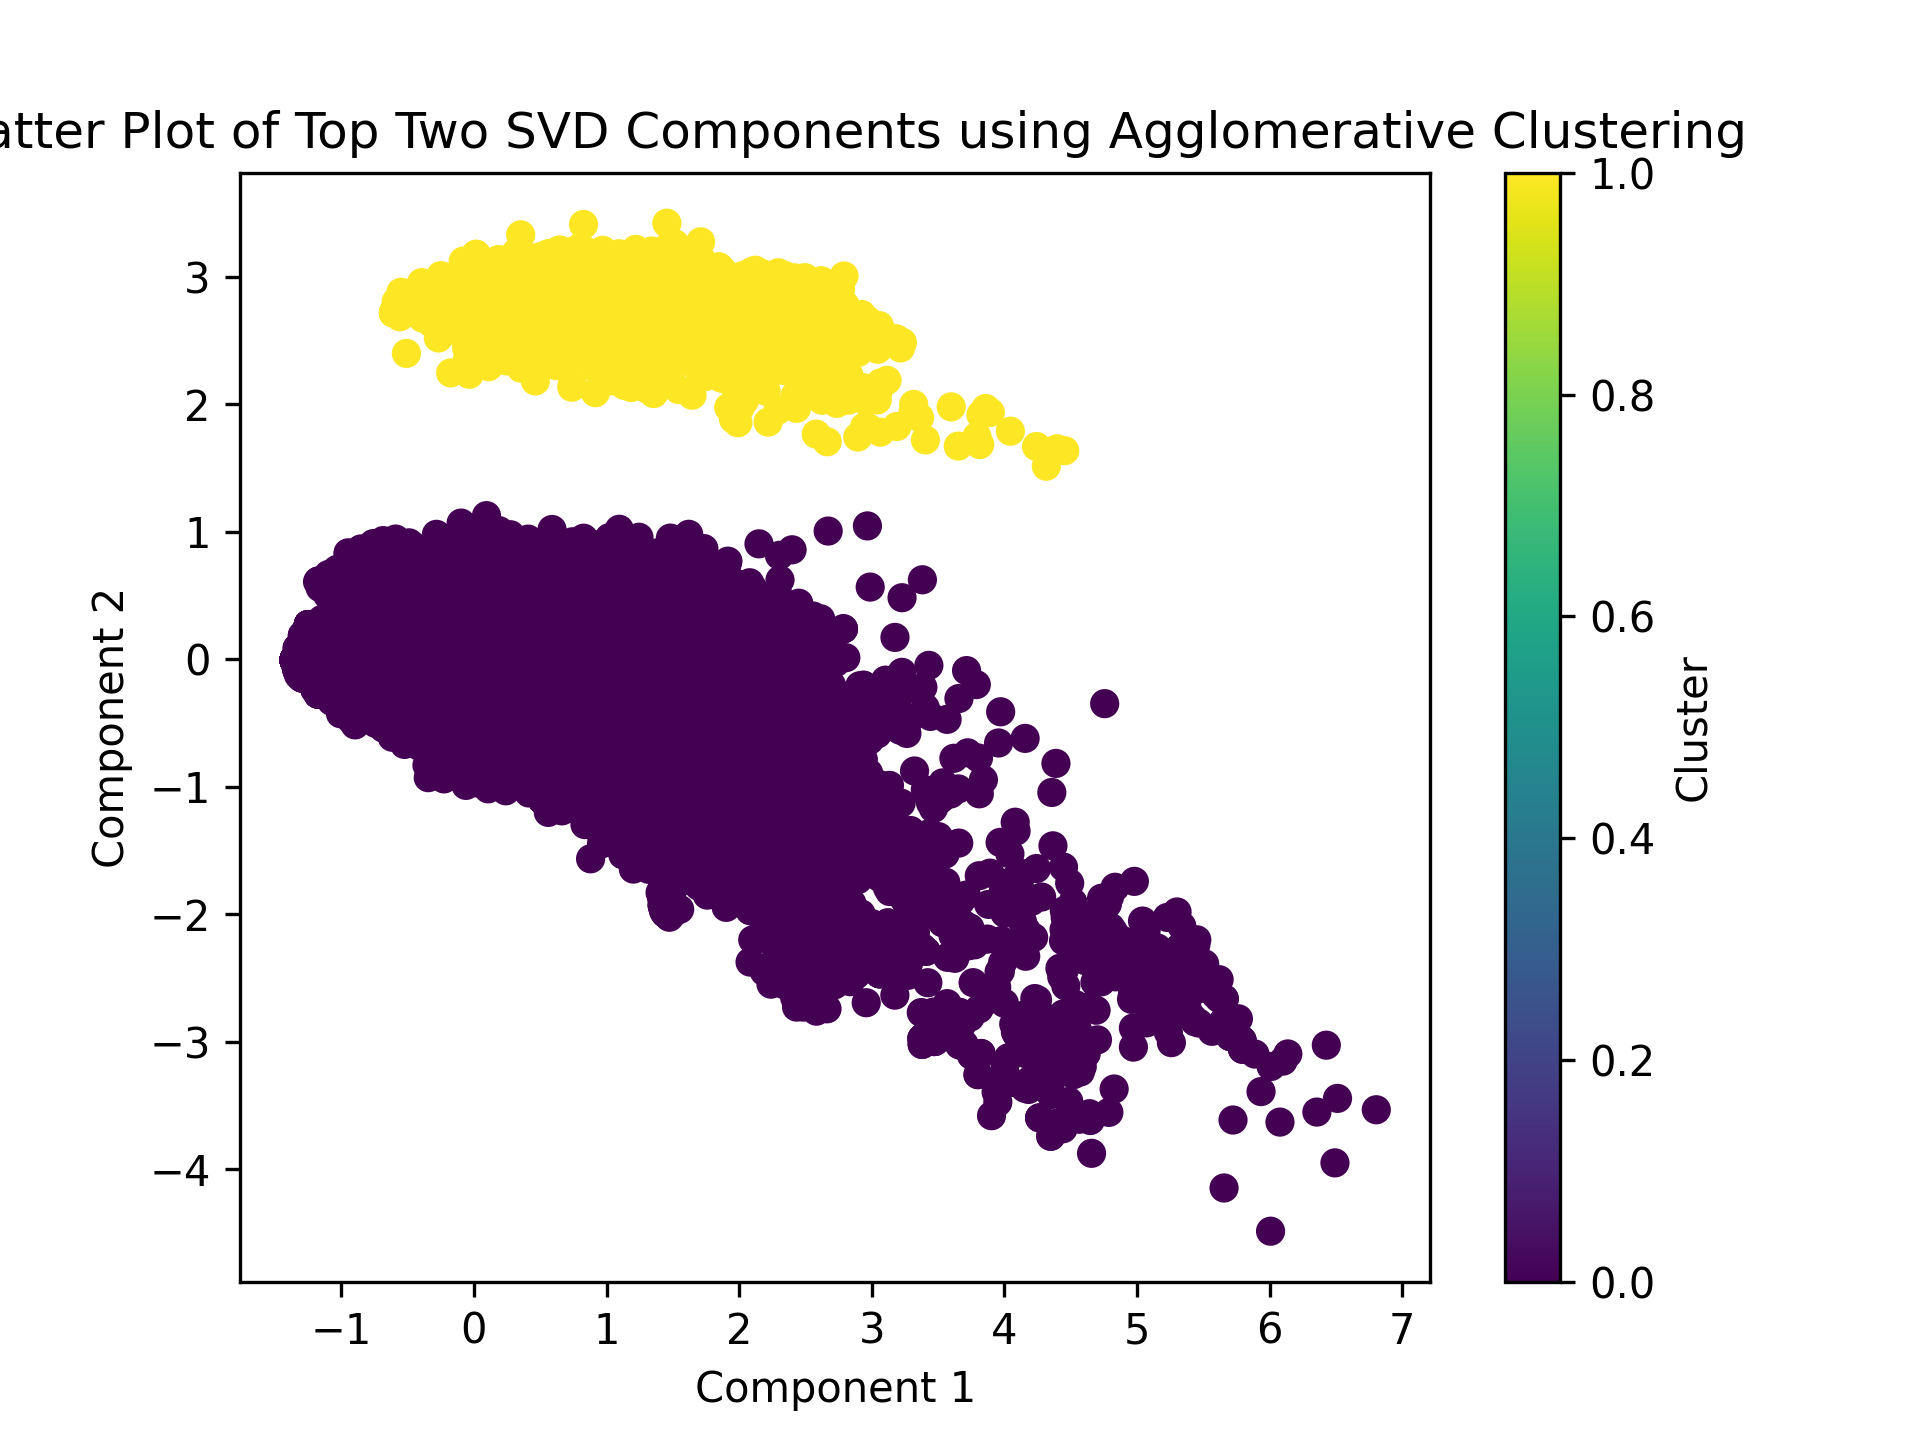
\includegraphics[width=\columnwidth]{C:/GitHub/DataScienceMachineLearning/wk_09/plots/AgglomerativeClustering.png}
    \caption{Aggloromerative Hierarchial Clustering}
\end{figure}

\vspace{1em}

\noindent When we look at figure 6, the clustering here looks much better. This is because there is clear separation between the clusters and aggloromerative
clustering is much better suited towards non-convex clusters. 

\subsection{The Confusion Matrix Heatmap}
Using the results of the aggloromerative hierarchial clustering model, we at last generate a confusion matrix to compare the ham / spam labels to the cluster
labels using the confusion matrix that we have generate as shown in Figure 7.

\begin{figure}[H]
    \centering
    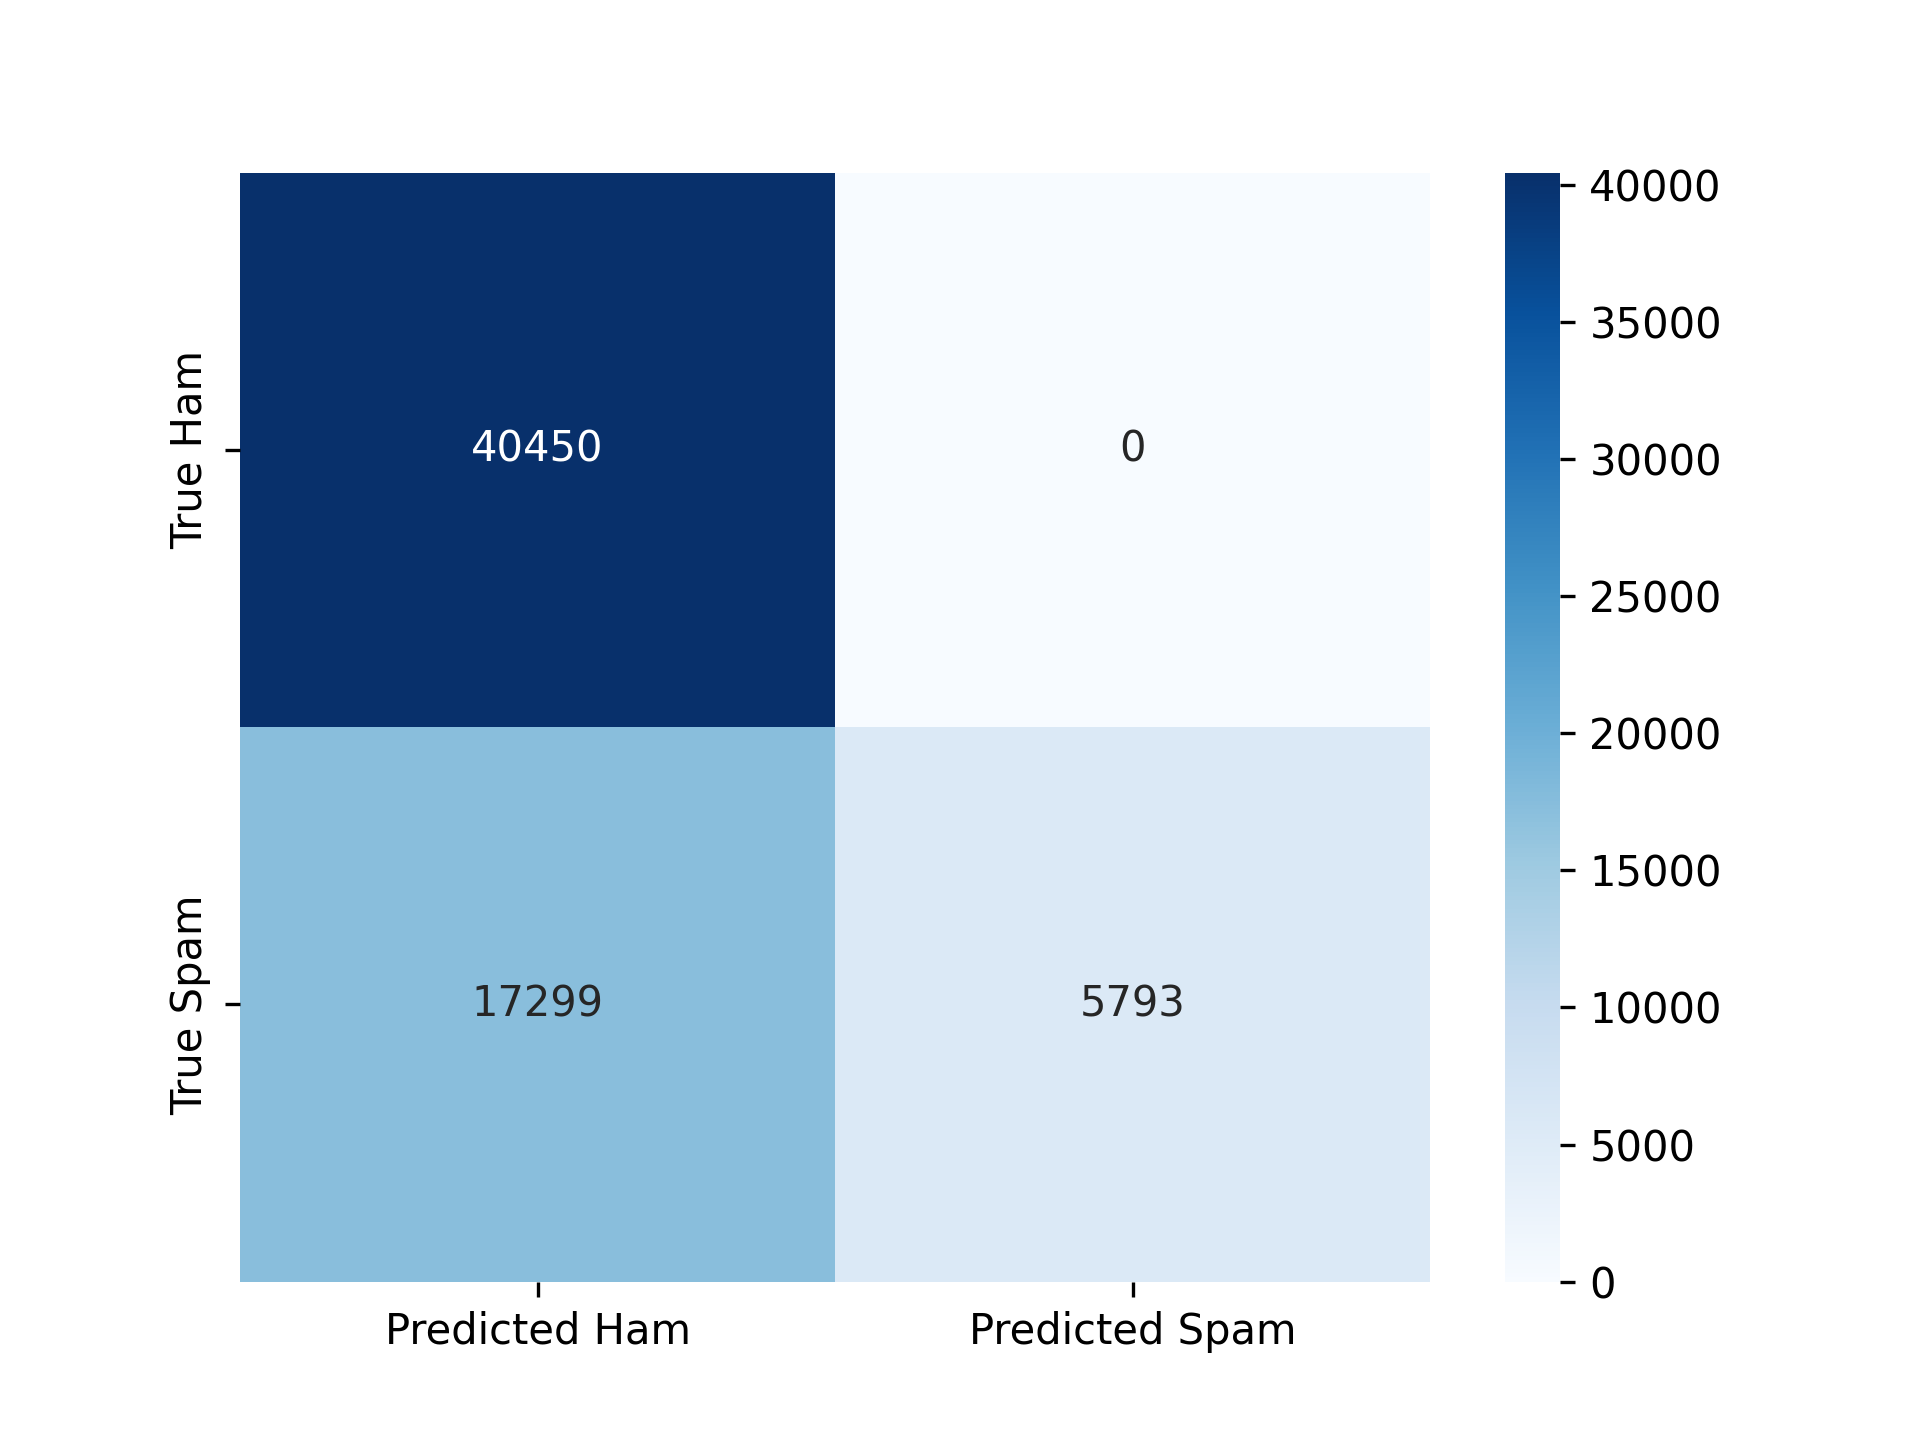
\includegraphics[width=\columnwidth]{C:/GitHub/DataScienceMachineLearning/wk_09/plots/HeatMap.png}
    \caption{HeatMap of Confusion Matrix}
\end{figure}

\newpage

\noindent The results of the heat maps shows us that the number of true positives (emails correctly identified as spam) is 5793. The number of true negatives
(emails correctly identified as ham) is 40450. When it came to false positives (ham incorrectly identified as spam) we got 0 and false negatives (spam 
incorrectly identified as ham) is 17,299. \\

\noindent Zero false positives implies that every positive results identified by the clustering model was incorrect, which is a great result to have. However, 
a few false negatives means that the model misses actual positives at times. We can now use the results from the confusion matrix to calculate the F1 score,
which measures how well the clusters match the actual spam vs ham classification, as it balances both precision and recall as shown in equation 1.

\begin{equation}
    \text{F1 Score} = 2 \times \frac{\text{Precision} \times \text{Recall}}{\text{Precision} + \text{Recall}}
    \label{eq:f1}
\end{equation}

\noindent When we calculate the F1 score, we get 0.42 when rounded to two decimal places. Since our F1 score is close to 0.5, the clusters match the 
categories partially.


\section{Discussion}
In this last section, we discuss the conclusions from the results we've obtained and summarize what we've understood from the experiments that we've 
conducted.

\subsection{Understanding the Dataset}
When we first converted the json files into a pandas data frame, we wanted to look at the features that made up the data frame. The names of the features
were \texttt{category}, \texttt{to\_address}, \texttt{from\_address}, \texttt{subject} \& \texttt{body}. When we use \texttt{.info()} to know about the data 
types of the features, they all appear to be objects, however, there is more to that. The feature \texttt{category} is categorical as there are only two 
unique values, which makes it exception. The rest of the features are objects because there are simply bodies of text. 

\subsection{The Feature Matrix}
Now, we look at the feature matrix that we produced and look at the key statistics, such as the number of rows and columns, non-zero entries and the sparsity
ratio. We also explain the structure and meaning of the matrix, and provide an estimate of the memory usage.

\subsubsection{Rows and Columns of the Feature Matrix}
When we create a feature matrix by using \texttt{fit\_transform()} from \texttt{CountVectorizer}, we can see that the matrix consists of a total of 63542
rows and 32144 columns. When we look at the number on non-zero entries in the matrix, we get 6388795 non-zero entries. Non-zero entries refers to the 
positions in the matrix where the value is not zero. It is simply counting how many times a word appears in any email.

\subsubsection{Calculating the Sparsity Ratio}
When it comes to calculating the sparsity ratio, we calculate it by 100 * (number of non-zero entries / maximum possible entries). Using equation 2 below, we
get the sparsity ratio as 0.3127938123616995.

\begin{equation}
    \text{Sparsity} = 100 \times \left(\frac{\text{Non-zero entries}}{\text{Total entries}} \right)
\end{equation}

\subsubsection{The Meaning Behind The Feature Matrix}
When we look at the feature, the number of rows are the number of emails, from 0 to 63541 emails. The number of columns are the words in the emails that appear
atleast more than 10 emails. We then cross-check these words against the emails to see if the word is present in the email. If the word is present the email,
we use a binary value of 1 to indicate it as true, else 0 to indicate it as false.

\subsubsection{The Compressed Row Format}
Lastly, the vectorize we use returns a sparse matrix in CSR. Since we assume that the sparse matrix uses one 32-bit and one 32-bit integer for each non-zero
entry and one 32-bit integer for each row. When we calculate the memory usage as shown in equation 3, we get the memory as near 49 MB.

\begin{equation}
    \text{Total Memory Usage} = 8 \times \text{nnz} + 4 \times (m + 1)
\end{equation}

\subsection{A Closer Look at Dimensionality Reduction}
When it came to performing dimensionality reduction, we used \texttt{fit\_transform} to create a new matrix with 10 components. In order to find the components
with the largest explained variance ratios, we found that it was component 0 and 1 which had a explained variance ratio of 0.057 and 0.028 respectively.

\subsection{A Closer Look at Clustering}
In this section, we look at the clusters we've created using two unsupervised learning models in great detail and discuss what we did.

\subsubsection{Cluster Assignment Analysis}
Looking at the clustering algoirthm that we used (agglomerative hierarchial clustering), we observe a convex structure to these clusters. It is evident that
the data points naturally form two distinct clusters. When we compare the clusters with the actual labels, we believe that clustering will allow for 
recovering the label as the clustering forms two distinct groups.

\subsubsection{Choice of Clustering Algorithm}
When it came k-means clustering, it appears to show irregular cluster shapes. This led to overlap between the two clusters, and where one cluster is bigger
than the other. When it came to using aggloromerative hierarchial clustering, there is a clear separation between the clusters, and we know this happend 
because it can handle non-convex clusters well. Because there is a clear separation between the clusters, it made sense to go with the aggloromerative 
hierarchial clustering algorithm.

\subsubsection{Application of Transformations}
When it came to application of transformations prior to clustering, we applied principal component analysis as well as standardizing. It is important to
standard the feature matrix so that each feature has a mean of zero and a standard deviation of one, which means that no feature is dominant when we use
a machine learning model on it. We use PCA because it helps to reduce the number of features while retaining most of the data's variance. This is beneficial
because it prevents overfitting in the model and improved the performance of the machine learning model.

\subsubsection{The Ham \& Spam Labels vs Cluster Labels}
Given the 5,793 true positives where spam emails are correctly clustered as spam and 17,299 false negatives where spam emails are clustered as ham, this 
means that the spam messages are split across both clusters. But, because we have 0 false positives, where no ham emails were misclassified as spam, this 
means any cluster that contains any spam emails will only have spam emails, with no ham emails in it. As a result, our clustering was partially successful, 
and we can back this with the F1 score that we calculated as well as the 17,299 spam emails that were all false negatives.

\subsection{The Top 200 Words}
Skimming through the top 200 words in each cluster, we wanted to identify any patterns possible. To achieve this, we decided to take the 200 words from each
cluster and generate two word clouds as shown in Figure 8 and 9 respectively. \\

\noindent When we look at the terms in Figure 8, we can see that there are statistical terms being used, such as biostatistical and bioinformation. There are
also R functions mentioned, such as anova. Overall, it seems like there are academic terminology being used, which appears to stem from the biology or 
biomedical field. As a result, we can determine that the words from this cluster comes from the ham cluster. \\

\noindent When we look at the terms in Figure 9, we see words such as acc, abating and aber, which are all words that suggest they are random words. It it 
worth noting that there are words which indicate violence, such as abduction and abducted. The violent nature of the words being used suggests to use that
these words originate from the spam cluster.

\newpage

\begin{figure}[H]
    \centering
    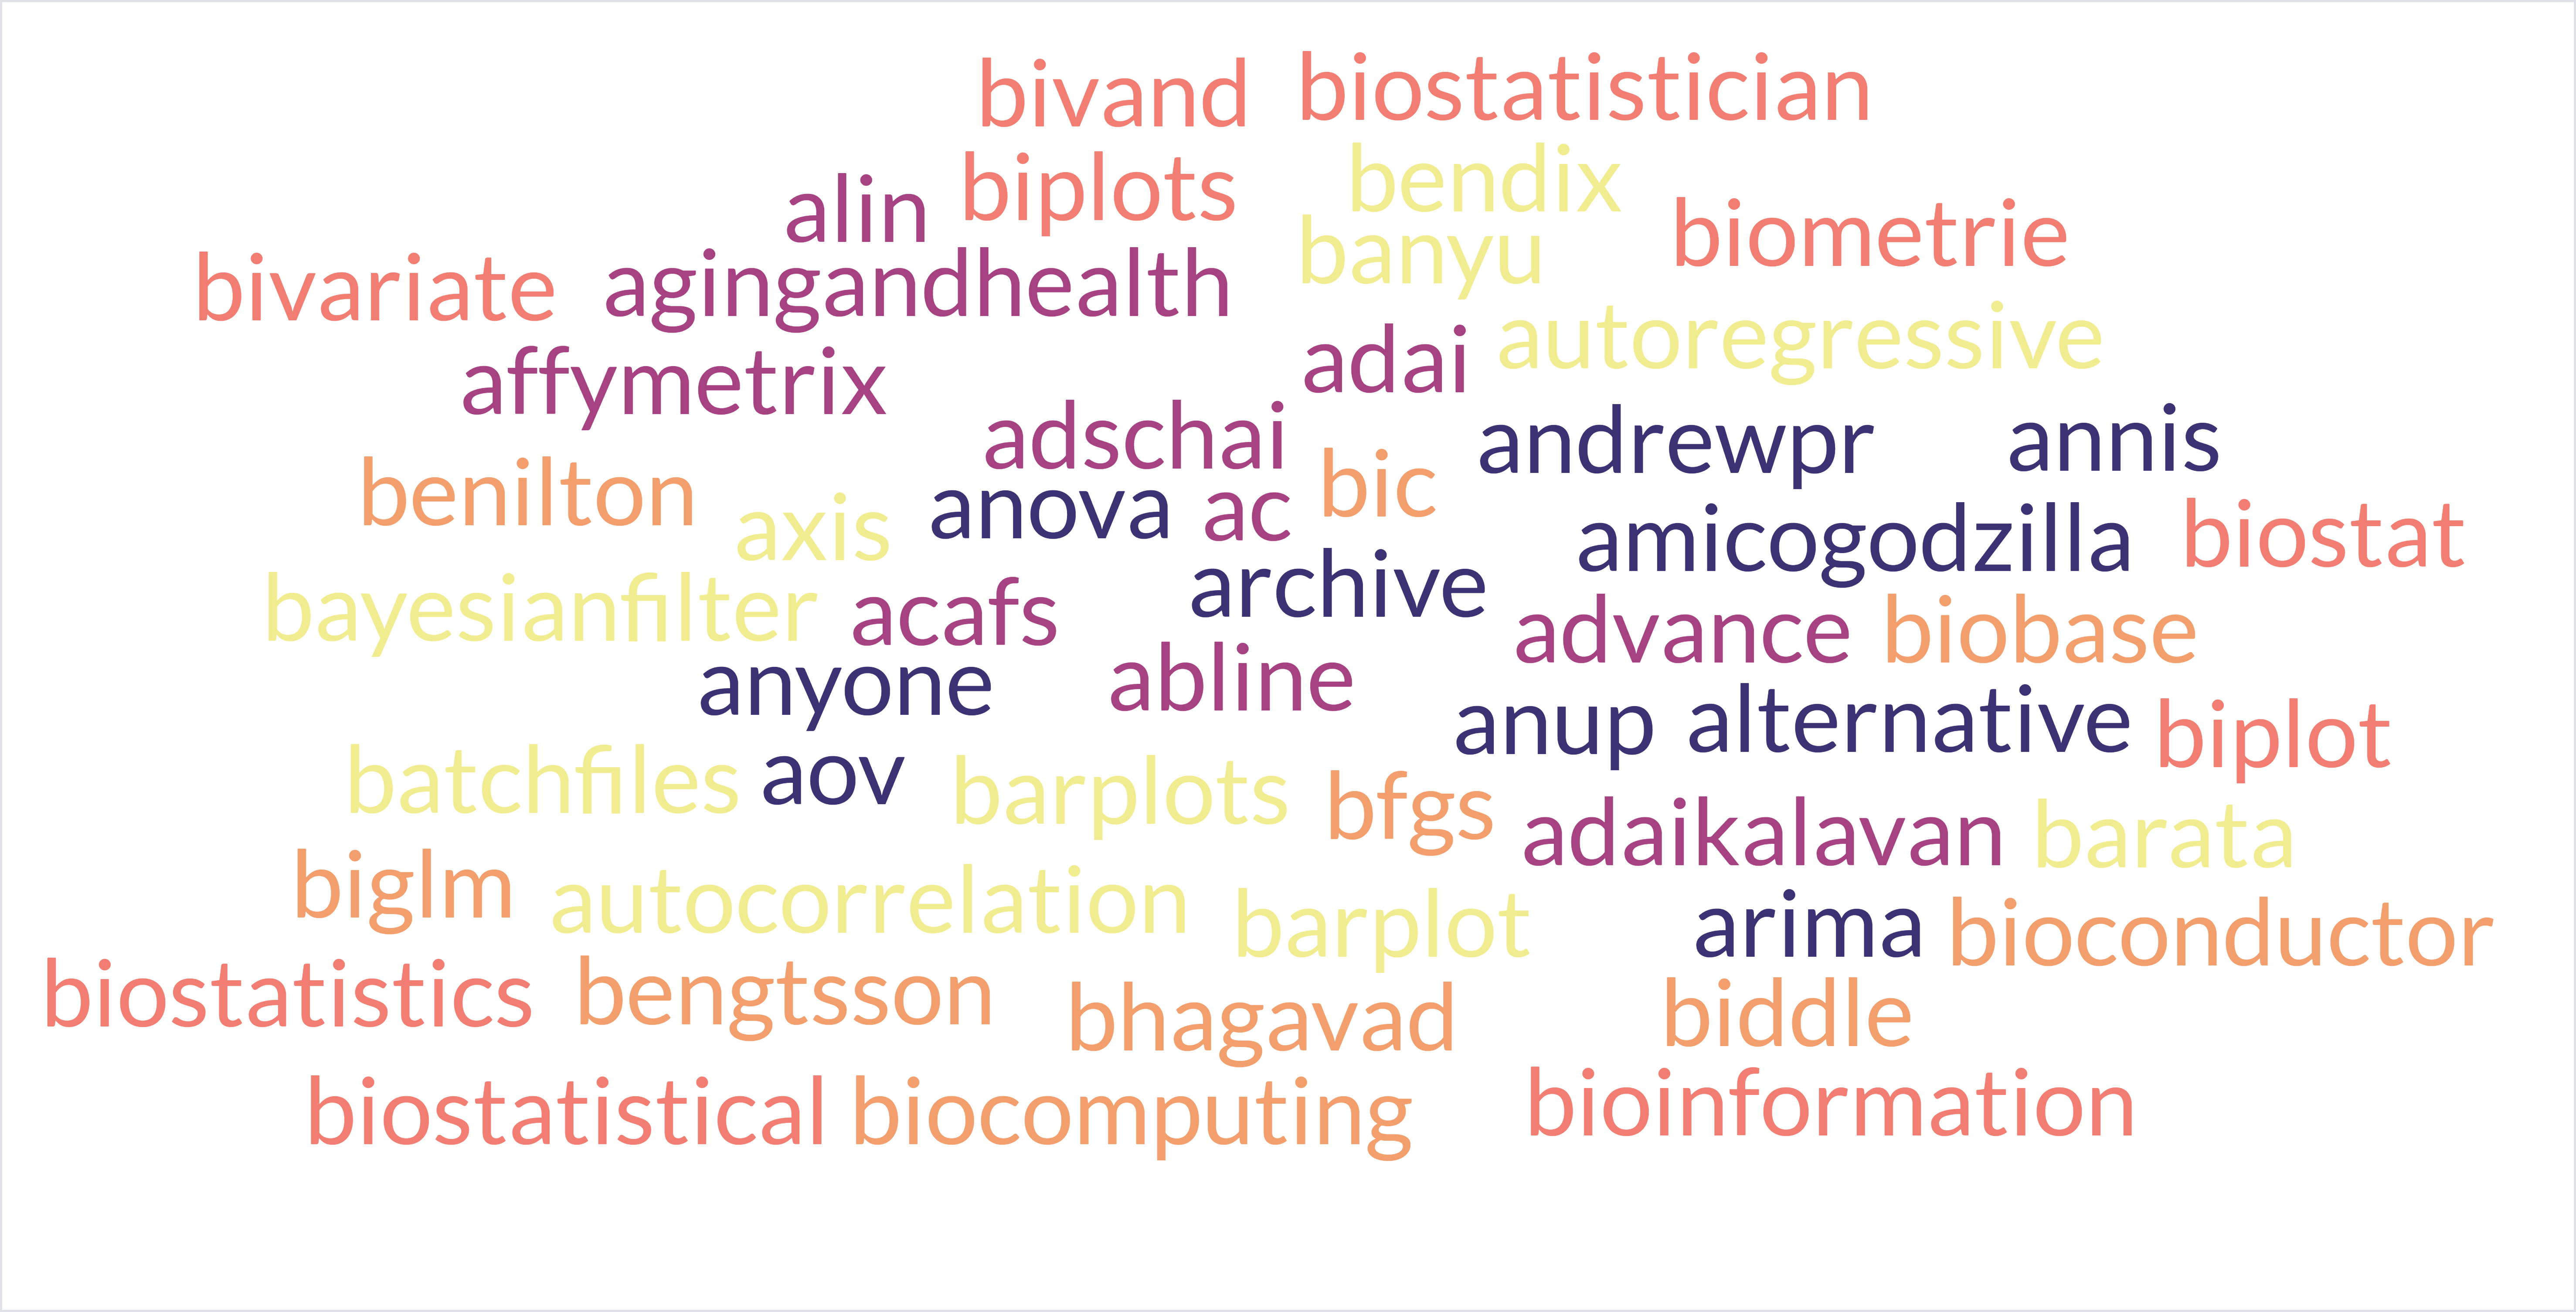
\includegraphics[width=\columnwidth]{C:/GitHub/DataScienceMachineLearning/wk_09/plots/HamCloud.png}
    \caption{Word Cloud for Cluster 1}
\end{figure}

\vspace{2em}


\begin{figure}[H]
    \centering
    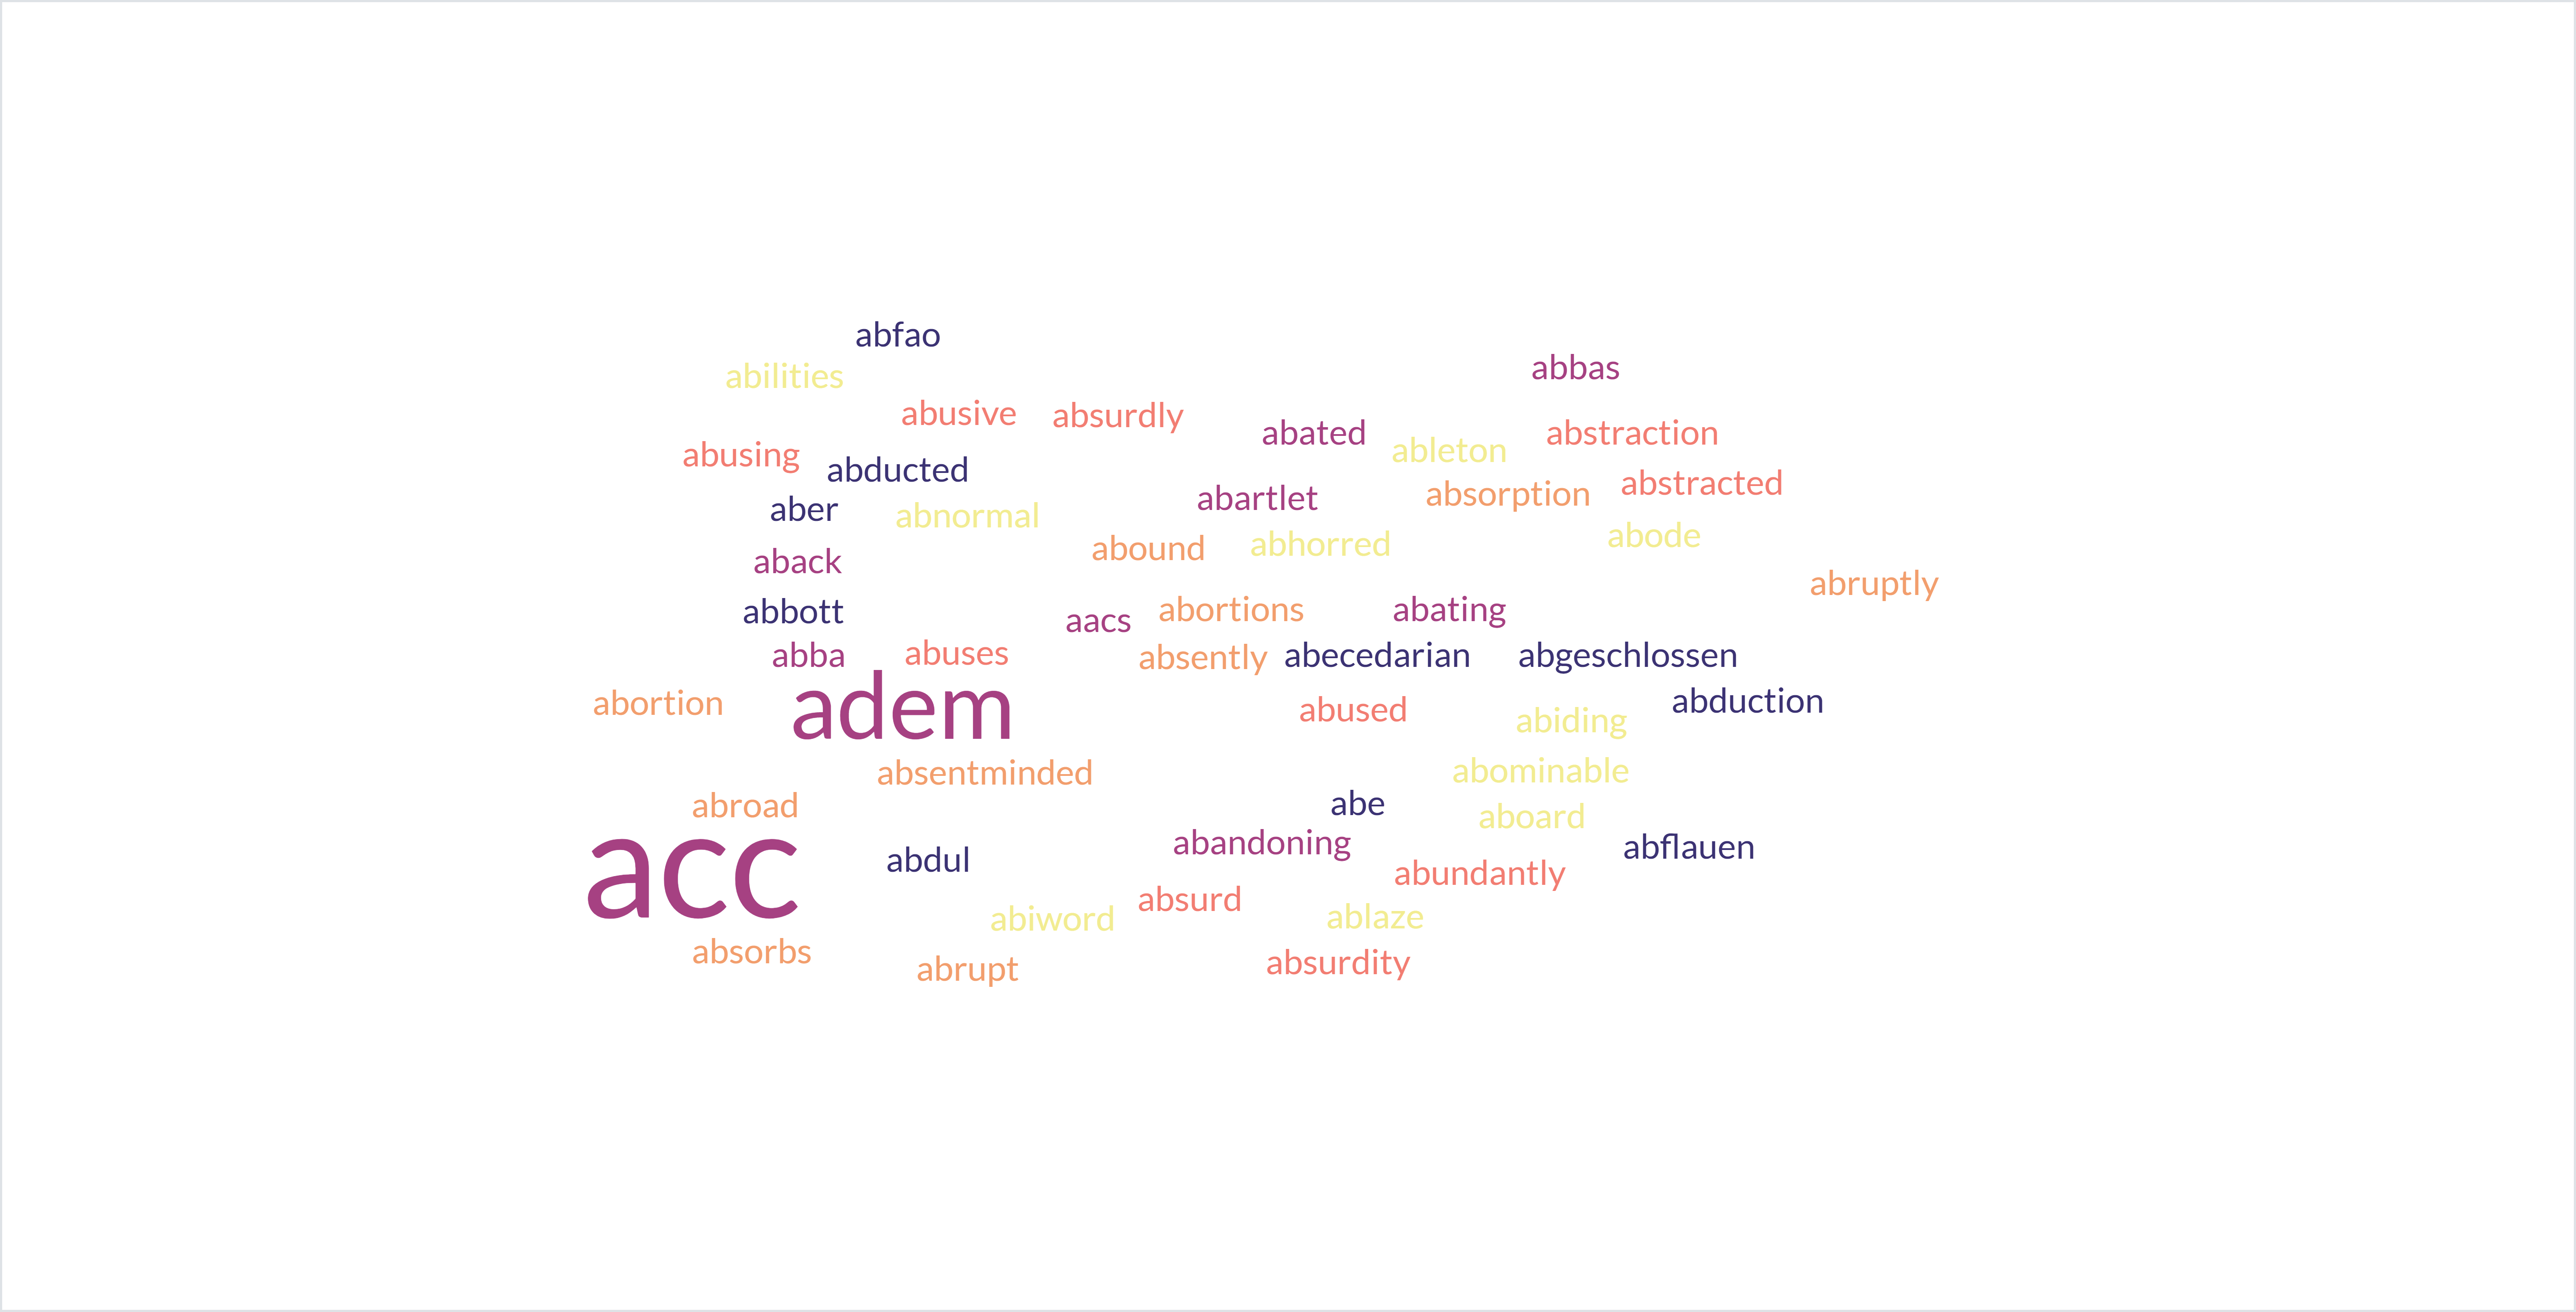
\includegraphics[width=\columnwidth]{C:/GitHub/DataScienceMachineLearning/wk_09/plots/SpamCloud.png}
    \caption{Word Cloud for Cluster 2}
\end{figure}

\end{document}